\begin{figure}[ht]
    \vspace{0.3cm}
    \centering
    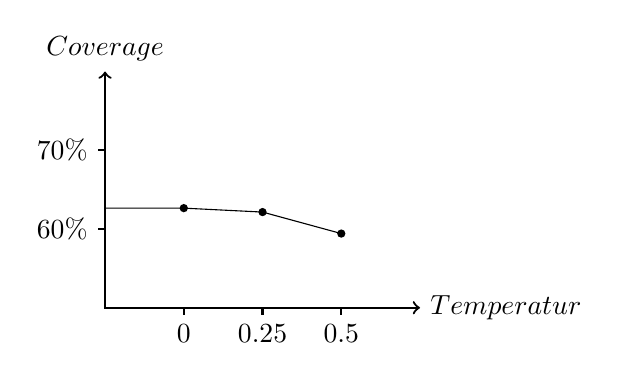
\begin{tikzpicture}
    \draw [<->,thick] (0,3) node (yaxis) [above] {$Coverage$}
        |- (4,0) node (xaxis) [right] {$Temperatur$};
    \draw (0,1.265) coordinate (a_1) -- (1,1.265) coordinate (a_2) -- (2,1.215) coordinate (a_3) -- (3, 0.942) coordinate (a_4);
    \draw[thick] (0, 1) -- (-0.09, 1) node[anchor=east] {60\%};
    \draw[thick] (0, 2) -- (-0.09, 2) node[anchor=east] {70\%};
    \draw[thick] (1, 0) -- (1, -0.09) node[anchor=north] {0};
    \draw[thick] (2, 0) -- (2, -0.09) node[anchor=north] {0.25};
    \draw[thick] (3, 0) -- (3, -0.09) node[anchor=north] {0.5};
    \coordinate (b) at (1,1.265);
    \fill[black] (a_2) circle (1.5pt);
    \fill[black] (a_3) circle (1.5pt);
    \fill[black] (a_4) circle (1.5pt);
    \end{tikzpicture}
    \caption{Einfluss der Temperatur auf die Coverage}
    \label{fig:temp}
\end{figure}